% Paper: Optimized GEMV Kernel for AMD Zen 3
% Format: FedCSIS / IEEEtran
\documentclass[conference]{IEEEtran}
\IEEEoverridecommandlockouts

% This package serves to balance the column lengths on the last page of the document.
\usepackage{pbalance}

%% to enable \thank command
\IEEEoverridecommandlockouts
%% The usage of the following packages is recommended
%% to insert graphics
\usepackage{graphicx}
% to typeset algorithms
\usepackage{algorithmic}
\usepackage{algorithm}
% to typeset code fragments
\usepackage{minted}
% to make an accent \k be available
\usepackage[OT4,T1]{fontenc}
% provides various features to facilitate writing math formulas and to improve the typographical quality of their output.
\usepackage[cmex10]{amsmath}
\interdisplaylinepenalty=2500
\usepackage{amssymb}
\usepackage{booktabs}
% for urls typesetting and breaking
\usepackage{url}
\usepackage{hyperref}
% for vertical merging table cells
\usepackage{multirow}


\title{High-Performance GEMV on AMD Zen~3 via Architecture-Specific AVX2/FMA Optimization}

\author{
\IEEEauthorblockN{Rafa{\l} Lenart}
\IEEEauthorblockA{0009-0007-8389-7835\\
Maria Curie-Sk{\l}odowska University\\
Lublin, Poland\\
Email: rafa.lenart12@gmail.com}
\and
\IEEEauthorblockN{Beata Bylina}
\IEEEauthorblockA{0000-0002-1327-9747\\
Maria Curie-Sk{\l}odowska University\\
Lublin, Poland\\
Email: beata.bylina@umcs.pl}
\and
\IEEEauthorblockN{Jaros{\l}aw Bylina}
\IEEEauthorblockA{0000-0002-0319-2525\\
Maria Curie-Sk{\l}odowska University\\
Lublin, Poland\\
Email: jaroslaw.bylina@umcs.pl}
}


\begin{document}
\maketitle

\begin{abstract}
The General Matrix-Vector Multiply (GEMV) is a fundamental Level-2 BLAS operation
appearing throughout scientific computing and numerical linear algebra.
GEMV is inherently memory-bound, making effective cache use the dominant optimization factor.

We present a hand-optimized GEMV kernel for AMD Zen~3, implemented using AVX2 and
FMA intrinsics. Our single-threaded kernel (ZenGEMV) processes 4~rows simultaneously
with dual accumulators per row, creating 8~independent FMA chains that fully saturate
the Zen~3 pipeline. Benchmarked against OpenBLAS~0.3.31 and AOCL-BLAS~5.2.0 on an
AMD Ryzen~5~5600, ZenGEMV achieves up to $1.37\times$ speedup over OpenBLAS and
$1.20\times$ over AOCL-BLAS. Our parallel variant (ZenGEMV-P) achieves up to
$3.22\times$ speedup over OpenBLAS on small matrices.

We analyse why dispatch overhead, suboptimal accumulator strategies, and generic
design choices in general-purpose BLAS libraries leave performance gains available in
architecture-specific workloads.
\end{abstract}

\begin{IEEEkeywords}
GEMV, BLAS, AVX2, FMA, AMD Zen~3, SIMD, OpenMP
\end{IEEEkeywords}


%=============================================================
\section{Introduction}
%=============================================================

\IEEEPARstart{T}{he} Basic Linear Algebra Subprograms (BLAS)\cite{blas} are a widely adopted set of standardized interfaces
for vector (Level-1), matrix-vector (Level-2), and matrix-matrix (Level-3) operations. Among these, the Level-2
BLAS operation GEMV (General Matrix-Vector Multiplication) computes
$\mathbf{y} \leftarrow \alpha A\mathbf{x} + \beta\mathbf{y}.$
In computational science, GEMV serves as a core subprogram in a broad range of algorithms, including:
\begin{enumerate}
  \item Dense matrix factorizations such as Householder QR and Hessenberg reduction\cite{golub2013}, where each step of the unblocked algorithm applies a Householder reflector via a GEMV on the trailing submatrix.
  \item Token generation in Large Language Models (LLMs), where each decoding step reduces to a sequence of GEMV operations.\cite{waferllm}
  \item Recurrent neural network (RNN/LSTM) inference\cite{grnn}, where each time step performs dense matrix--vector multiplications with the weight matrices.
\end{enumerate}

GEMV is fundamentally memory-bound. For an
$M \times N$ matrix, the operation performs $2MN$ floating-point operations while
transferring $O(MN)$ bytes of matrix data, yielding an operational intensity of
approximately 0.25~FLOP/byte---well below the ridge point of modern
processors (we derive this value formally in
Section~\ref{sec:gemv_op}). This memory-bound nature means that the primary
optimization target is not compute throughput but rather effective use of the
memory hierarchy and minimization of pipeline stalls.

Production BLAS libraries such as OpenBLAS\cite{openblas} and
AOCL-BLAS\cite{aoclblas} are designed for generality: they handle arbitrary
strides, all combinations of transpose and conjugate operations, and dynamically
select microkernels based on detected hardware. This generality introduces a
roughly constant dispatch overhead per call. While this overhead is amortized
away for large matrices in both GEMM and GEMV, it becomes significant for tiny
and small matrices where the compute-to-overhead ratio is low---a regime in
which GEMV is frequently invoked, for example during per-token decoding in LLM
inference.

This paper investigates whether a hand-optimized kernel, tailored to a specific
microarchitecture and constrained use case, can outperform these general-purpose
libraries. Our contributions are:
\begin{enumerate}
  \item An optimized single-threaded GEMV kernel (ZenGEMV) using AVX2 (Advanced Vector Extensions 2)\cite{avx2} and FMA (Fused Multiply-Add)\cite{fma}
      intrinsics with dual accumulators that fully saturate the Zen~3\cite{zen3} FMA
      pipeline.
\item A parallel variant (ZenGEMV-P) with row-parallel decomposition using
      manual thread work division aligned to SIMD boundaries.
\item A detailed source-level analysis of OpenBLAS and AOCL-BLAS GEMV overhead,
      explaining where and why performance is lost.
\end{enumerate}


%=============================================================
\section{Background and Related Work}
\label{sec:gemv_op}
%=============================================================

The GEMV operation computes:
\begin{equation}
\mathbf{y} \leftarrow \alpha A \mathbf{x} + \beta \mathbf{y}
\label{eq:gemv}
\end{equation}
where $A \in \mathbb{R}^{M \times N}$ is a matrix with $M$~rows and $N$~columns,
$\mathbf{x} \in \mathbb{R}^N$ is the input vector,
$\mathbf{y} \in \mathbb{R}^M$ is the output vector, and $\alpha, \beta$ are
scalars. The dimensions $M$ (rows) and $N$ (columns) determine both the
computational cost and the memory footprint of the operation.

The operation requires $2MN$ floating-point operations---one multiply and one add
per element of~$A$. The total data movement is $(MN + N + 2M) \times 8$ bytes
for double-precision (the matrix~$A$, input vector~$\mathbf{x}$, and the
output vector~$\mathbf{y}$ read and written), giving an operational intensity\cite{roofline} of:
\begin{equation}
\text{OI} = \frac{2MN}{8(MN + N + 2M)} \approx \frac{1}{4} \text{ FLOPs/byte}
\label{eq:ai}
\end{equation}
for large $M$ and $N$, where the vector terms become negligible relative to the
matrix. This makes GEMV memory-bound on all modern
architectures.

Our target platform is the AMD Ryzen~5~5600, based on the Zen~3
microarchitecture. The relevant parameters are sourced from the AMD Software
Optimization Guide\cite{amdsog} and Agner Fog's instruction
tables\cite{fog2011instruction} and microarchitecture guide\cite{fog2017microarchitecture}:

\begin{itemize}
\item \textbf{Cache hierarchy:} 32\,KiB L1d (8-way, latency 4 clocks) per core,
      512\,KiB L2 (8-way, latency 14 clocks) per core, 32\,MiB shared L3 (16-way,
      latency 47 clocks).
\item \textbf{Execution units:} Two 256-bit FMA units capable of
      executing \texttt{vfmadd} instructions.
\item \textbf{FMA pipeline:} Each \texttt{vfmadd231pd} instruction has a
      4-cycle latency but the two FMA units can accept a new instruction every
      cycle (2-per-cycle throughput). Because the pipeline is
      4~stages deep, an FMA result is not available for 4~cycles after issue.
      To avoid stalls, the code must maintain independent operations that can
      fill the pipeline while earlier results are computed. With 2~units each
      having 4-cycle latency, the minimum number of independent FMA operations
      needed for full utilization is $4 \times 2 = 8$.
\item \textbf{Peak throughput:}
      $2\ \text{FMA} \times 4\ \text{doubles} \times 2\ \text{ops} \times
      4.4\ \text{GHz} = 70.4\ \text{GFLOPS/core}$ at maximum boost clock.
      This value is the theoretical peak.
\item \textbf{Memory bandwidth:} The Ryzen~5~5600 uses a DDR4 memory controller.
      Our test system is equipped with DDR4 3200 MT/s CL16 modules,
      providing a theoretical peak of 51.2 GB/s in dual-channel mode.
      This value was calculated using an online tool.\cite{ramcalc}
\end{itemize}

The Roofline model\cite{roofline} provides an upper bound on attainable
performance as a function of a kernel's operational intensity (OI, the ratio of
floating-point operations to bytes transferred) and the system's memory bandwidth
(BW, in GB/s):
\begin{equation}
P_{\max} = \min(P_{\text{peak}},\ \text{BW} \times \text{OI})
\label{eq:roofline}
\end{equation}

For GEMV with $\text{OI} \approx 0.25$~FLOP/byte, the theoretical maximum
depends on which level of the memory hierarchy serves the data. The practical
bandwidth at each cache level is derived from the sustained transfer width per
cycle at the sustained core frequency of 4.4\,GHz:
\begin{itemize}
  \item \textbf{L1d:} The L1d cache supports up to two 256-bit (32-byte) loads and one 128-bit (16-byte) load simultaneously which combined with the 4.4 GHz boost clock gives
      $2 \times 32 \times 4.4 + 1 \times 16 \times 4.4 = 352$\,GB/s theoretical throughput; practical
      throughput is likely less than $\sim$281.6\,GB/s due to at least one port being usually dedicated to store operations.\cite{amdsog}
\item \textbf{L2:} The L2 to L1 data path delivers 32~bytes/cycle to L1, giving
  $32 \times 4.4 = 140.8$\,GB/s;\cite{amdsog}
\item \textbf{L3:} The per-core L3 read bandwidth was measured empirically using
      the \textit{bandwidth} tool by Zack Smith~\cite{bandwidth} on sequential
      256-bit reads. Buffer sizes in the L3-resident range (1\,MB--16\,MB)
      yielded $\sim$106\,GB/s sustained read bandwidth. The raw measurement
      output is shown in Fig.~\ref{fig:bandwidth}.
\item \textbf{DRAM:} DDR4-3200 dual-channel provides
      $3200 \times 8 \times 2 = 51.2$\,GB/s theoretical. The
      \textit{bandwidth} microbenchmark reports $\sim$42\,GB/s for
      sequential 256-bit reads from a single core
      (Fig.~\ref{fig:bandwidth}), but GEMV's highly regular streaming
      access pattern enables more effective hardware prefetching; our
      measured GEMV throughput on DRAM-resident data
      (Section~\ref{sec:results}) is consistent with the full 51.2\,GB/s
      ceiling, which we adopt as the practical DRAM bandwidth.
\end{itemize}
The GEMV ceiling at each level is then computed from Equation~(\ref{eq:roofline})
as $\text{BW} \times \text{OI}$ (e.g., $267 \times 0.25 = 66.75$~GFLOPS for
L1d). Table~\ref{tab:ceilings} summarizes these values.


\begin{table}[tbp]
\centering
\caption{Bandwidth ceilings and GEMV performance limits per memory level
(OI~$= 0.25$~FLOP/byte).}
\label{tab:ceilings}
\begin{tabular}{@{}l c c c@{}}
\toprule
\textbf{Memory Level} & \textbf{Practical BW} &
  \textbf{GEMV Ceiling} & \textbf{Size} \\
\midrule
L1d   & 267\,GB/s  & 66.8\,GFLOPS & 32\,KB  \\
L2    & 132\,GB/s  & 33.0\,GFLOPS & 512\,KB \\
L3    & 106\,GB/s  & 26.5\,GFLOPS & 32\,MB  \\
DRAM  & 51.2\,GB/s & 12.8\,GFLOPS & ---     \\
\bottomrule
\end{tabular}
\end{table}

\begin{figure}[tbp]
\centering

\includegraphics[width=\linewidth]{bandwidth.pdf}
\caption{Memory bandwidth measured with the \textit{bandwidth}
tool~\cite{bandwidth} on the AMD Ryzen~5~5600 for sequential reads, writes,
nontemporal (NT) operations, and copies at 64/128/256-bit widths. The shaded
regions mark cache levels: L1d ($\sim$267\,GB/s peak read), L2 ($\sim$132\,GB/s),
L3 ($\sim$106\,GB/s), and DRAM ($\sim$42\,GB/s).}
\label{fig:bandwidth}
\end{figure}

When the working set fits in cache, the effective bandwidth increases
dramatically, enabling much higher throughput for small to medium matrices
than the DRAM-bound prediction would suggest. Fig.~\ref{fig:roofline} shows the
roofline diagram with our measured ZenGEMV performance for each benchmark preset,
demonstrating how cache residency determines the reachable performance level.


\begin{figure*}[tbp]
\centering
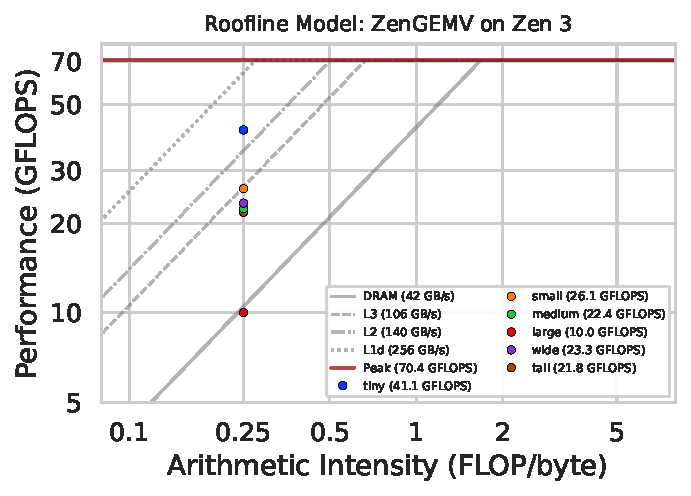
\includegraphics[width=\linewidth]{roofline.pdf}
\caption{Roofline model for Zen~3. Diagonal lines show memory bandwidth
ceilings from DRAM through L1d; horizontal colored lines mark the GEMV-specific
performance ceilings at each cache level ($\text{BW} \times 0.25$).
Points show measured ZenGEMV performance at each preset's operational intensity,
illustrating how cache residency determines the attainable performance level.}
\label{fig:roofline}
\end{figure*}

\subsection{Related Work}

\textbf{OpenBLAS}\cite{openblas} descends from GotoBLAS\cite{gotoblas} and
provides architecture-specific assembly kernels. Its GEMV implementation
uses column blocking with \texttt{NBMAX=2048}. All ZEN generations share
the microkernel \texttt{dgemv\_t\_microk\_haswell-4.c}, which processes
4~rows simultaneously with a single accumulator per row.

\textbf{AOCL-BLAS} is AMD's optimized fork of the BLIS\cite{blis} framework,
decomposes GEMV operations into fused Level-1 microkernels with a configurable
fuse factor (detailed in Section~\ref{sec:blis}), and includes a Zen~3 tuned
configuration in version~5.2.0.

The ATLAS project\cite{atlas} pioneered empirical auto-tuning for BLAS,
searching blocking parameters and code transformations to maximise cache
efficiency. Hassan\cite{hassan2017gemv} demonstrates that hand-written
AVX SGEMV kernels can outperform Intel MKL on multicore x86 processors;
Fog\cite{fog2011instruction,fog2017microarchitecture} documents detailed
instruction latencies and throughput for x86 microarchitectures, which informed
our kernel design.

On the GPU side, Abdelfattah et~al.\cite{kblas} present KBLAS, an optimized
library for dense matrix--vector multiplication on NVIDIA GPUs. Their
double-buffering technique overlaps data movement with computation, and
collaborative thread-block processing with atomic operations yields up to 60\%
speedup over cuBLAS. A subset of the KBLAS kernels have been integrated into
NVIDIA's cuBLAS.

Liang and Zhang\cite{liang2016gemv} specifically target Intel
AVX processors, combining prefetching strategies, AVX intrinsics with loop
unrolling, and OpenMP parallelization to achieve 5--10\% improvements over Intel
MKL, GotoBLAS, and ATLAS. Their work is directly comparable to ours, but targets
an Intel microarchitecture rather than AMD Zen~3. 

Singh and Bassoy\cite{singh2021gemv} take a complementary, portable approach: their
cache-blocked GEMV algorithms exploit L1/L2 blocking and FMA instructions
without hand-written assembly, relying on compiler optimizations to remain
competitive with MKL, BLIS, and OpenBLAS across multiple x86 platforms. In
contrast, our work deliberately specializes the microkernel for AMD Zen~3,
trading portability for higher utilization of the specific pipeline resources.


%=============================================================
\section{Implementation}
%=============================================================

The ZenGEMV kernel processes 4~rows of the matrix simultaneously in the inner
loop. This design is motivated by two key constraints of the Zen~3 FMA pipeline:

\begin{enumerate}
\item \textbf{FMA latency hiding:} Each \texttt{vfmadd231pd} instruction has
      4-cycle latency\cite{fog2011instruction}. With 2~FMA units executing per cycle, we need
      $4 \times 2 = 8$ independent FMA operations to keep both units fully occupied.
\item \textbf{reusing vector x:} Loading the $\mathbf{x}$ vector once and
      applying it to 4~rows reduces memory traffic.
\end{enumerate}

For each of the 4~rows, we maintain two independent accumulator registers
(\texttt{sum\_a} and \texttt{sum\_b}).

The main loop processes 16~elements per iteration (4~AVX2 loads of 4~doubles
each), alternating between accumulators~\texttt{a} and~\texttt{b}:

\begin{figure}[tbp]
\begin{minted}[fontsize=\scriptsize,frame=single,linenos]{c}
for (; j + 15 < cols; j += 16) {
    __m256d x0 = _mm256_load_pd(&x[j]);
    __m256d x1 = _mm256_load_pd(&x[j + 4]);
    __m256d x2 = _mm256_load_pd(&x[j + 8]);
    __m256d x3 = _mm256_load_pd(&x[j + 12]);

    sum0a = _mm256_fmadd_pd(
        _mm256_load_pd(&a0[j]),      x0, sum0a);
    sum0b = _mm256_fmadd_pd(
        _mm256_load_pd(&a0[j + 4]),  x1, sum0b);
    sum0a = _mm256_fmadd_pd(
        _mm256_load_pd(&a0[j + 8]),  x2, sum0a);
    sum0b = _mm256_fmadd_pd(
        _mm256_load_pd(&a0[j + 12]), x3, sum0b);
    // ... rows 1-3 follow the same pattern
}
\end{minted}
\caption{Inner loop of ZenGEMV (abbreviated, showing 1 of 4
rows).}
\label{lst:kernel}
\end{figure}

After the main loop, the dual accumulators are combined, and cleanup loops handle
remaining elements in groups of~8, 4, and finally scalar elements.
A horizontal sum reduction (\texttt{hsum\_pd}) converts each 256-bit accumulator
to a scalar result using \texttt{vextractf128} and \texttt{vhaddpd}\cite{avx2}.

Compiler hints including GCC's \texttt{always\_inline} and \texttt{hot}
attributes are used to ensure the kernel is inlined at the call site and marked
as performance-critical for the compiler's optimization heuristics.
The \texttt{\_\_restrict} qualifier on all pointer parameters enables the
compiler to assume no aliasing.

The compilation flags \texttt{-O3 -march=znver3 -mfma -mavx2 -flto}\cite{gccmanual}
enable architecture-specific code generation and link-time optimization.
We deliberately omit \texttt{-ffast-math}: the kernel is hand-vectorized
with intrinsics, so the compiler has no scope to apply unsafe reassociations,
and we measured no observable performance change from enabling it.

The ZenGEMV-P variant adds multi-threaded execution using OpenMP\cite{chandra2001parallel} with a
row-parallel decomposition strategy. Rather than using \texttt{\#pragma omp
parallel for}, which incurs per-iteration scheduling overhead, we use a single
\texttt{\#pragma omp parallel} region with manual work division:

\begin{figure}[tbp]
\begin{minted}[fontsize=\scriptsize,frame=single,linenos]{c}
#pragma omp parallel
{
    int nt  = omp_get_num_threads();
    int tid = omp_get_thread_num();
    int total_chunks = (rows + 3) / 4;
    int chunks_per   = total_chunks / nt;
    int extra         = total_chunks % nt;
    int start = tid*chunks_per + min(tid, extra);
    int end   = start + chunks_per + (tid < extra);
    process_row_range(start*4, min(end*4, rows),
                      cols, alpha, A, x, y);
}
\end{minted}
\caption{Thread work division in ZenGEMV-P.}
\label{lst:omp}
\end{figure}

Key design decisions:
\begin{itemize}
\item \textbf{4-row alignment:} Thread boundaries are aligned to 4-row groups,
      ensuring each thread uses the optimized 4-row kernel without partial
      processing at boundaries.
\item \textbf{No false sharing:} Each thread writes to a disjoint region of
      $\mathbf{y}$, eliminating cache-line contention.
\item \textbf{Adaptive thresholds:} Parallelization is only applied when
      the matrix has at least 128~rows and between $64\text{K}$ and $8\text{M}$
      elements. Below the lower threshold, thread creation overhead dominates.
      Above the upper threshold, DRAM bandwidth saturation makes additional
      threads counterproductive---measurements confirm that serial ZenGEMV
      outperforms the parallel variant in this regime, consistent with DRAM
      bandwidth saturation predicted by the roofline model (Fig.~\ref{fig:roofline}).
\end{itemize}


%=============================================================
\section{Analysis of Library Overhead}
%=============================================================

OpenBLAS GEMV processing involves several layers of overhead before reaching the kernel:

\begin{enumerate}
\item \textbf{CBLAS dispatch:} \texttt{cblas\_dgemv} validates the memory
      layout (\texttt{CblasRowMajor}/\texttt{CblasColMajor}) and transpose
      flag (\texttt{NoTrans}/\texttt{Trans}/\texttt{ConjTrans}), swapping
      $M$/$N$ and the transpose sense before forwarding to the Fortran-style
      \texttt{dgemv} entry point.
\item \textbf{Column blocking:} The implementation splits columns into blocks
      of \texttt{NBMAX=2048}, performing a horizontal reduction after each block.
      For matrices with $N > 2048$, this introduces additional reduction overhead
      and breaks the accumulation across blocks.
\item \textbf{Accumulator strategy:} OpenBLAS compiles all ZEN generations
      (ZEN through ZEN4) using the same shared microkernel
      \texttt{dgemv\_t\_microk\_haswell-4.c}, as determined by the preprocessor
      block in \texttt{kernel/x86\_64/dgemv\_t\_4.c}:
      \begin{minted}[fontsize=\scriptsize]{c}
#if defined(HASWELL) || defined(ZEN) || ...
#include "dgemv_t_microk_haswell-4.c"
#endif
      \end{minted}
      This kernel processes 4~rows simultaneously with a single accumulator
      per row, providing only 4~independent FMA chains. On Zen~3, 8~chains are needed for
      full utilization---this kernel leaves half the pipeline capacity unused.
\end{enumerate}

\label{sec:blis}
AOCL-BLAS uses an object-based design that provides clean abstractions at a
performance cost:

\begin{enumerate}
\item \textbf{Object dispatch:} \texttt{bli\_dgemv} constructs \texttt{obj\_t}
      structures (AOCL-BLAS's internal matrix/vector descriptors carrying dimensions,
      strides, and data pointers) and queries the hardware context
      (\texttt{cntx\_t}---a structure storing function pointers to
      architecture-specific microkernels along with cache and register blocking
      parameters for the target platform).
\item \textbf{Kernel abstraction:} AOCL-BLAS decomposes the GEMV operation into
      fused Level-1 primitives rather than implementing it monolithically.
      For the non-transpose case (\texttt{bli\_gemv\_unf\_var2}), it uses
      \texttt{AXPYF}---a fused \texttt{axpy} that performs $f$~scaled
      vector additions in a single pass, with fuse factor
      \texttt{b\_fuse=}$\texttt{BLIS\_AF}=5$ on Zen~3.
      For the transpose case (\texttt{bli\_gemv\_unf\_var1}), it uses
      \texttt{DOTXF}---a fused dot product that simultaneously computes
      the dot product of $\mathbf{x}$ against $f$~matrix rows, with
      \texttt{b\_fuse=}$\texttt{BLIS\_DF}=8$ on Zen~3.
      While this modularity enables code reuse across different BLAS operations,
      it prevents optimizations that span the entirety of the GEMV operation.
\item \textbf{Per-call initialization:} Every entry through the BLAS
      compatibility layer invokes \texttt{bli\_init\_auto()}---a library
      initialization guard---followed by parameter mapping
      (\texttt{bli\_param\_map\_netlib\_to\_blis\_trans}), dimension
      extraction, and stride setup before any computation begins. The
      kernel itself is invoked through a function pointer retrieved from
      \texttt{cntx} at runtime, adding an indirect call on every GEMV
      invocation.
\end{enumerate}

Despite these overheads, general-purpose libraries have advantages in certain
scenarios:

\begin{itemize}
\item \textbf{AOCL-BLAS on medium (1T):} AOCL-BLAS achieves 23.46~GFLOPS vs.\ our
      22.62~GFLOPS on $1024 \times 1024$. The AOCL-BLAS Zen~3 kernel configuration
      is well-tuned for L3-resident data, and its grouping strategies
      may provide better cache utilization at this specific size.
\item \textbf{Multi-threaded medium/tall presets:} OpenBLAS and AOCL-BLAS achieve
      competitive or slightly better multi-threaded performance on medium and
      tall presets, where the larger amount of work per call amortizes their
      thread-dispatching overhead.
\item \textbf{Generality:} Libraries handle arbitrary strides, non-contiguous
      memory layouts, complex alpha/beta combinations, and all transpose
      variants---features our kernel does not support.
\end{itemize}


%=============================================================
\section{Experimental Evaluation}
\label{sec:results}
%=============================================================

All experiments were conducted on an AMD Ryzen~5~5600 (6~cores, 12~threads,
Zen~3, base clock 3.5\,GHz, boost up to 4.47\,GHz) running Arch Linux with
kernel 6.18.7-zen1-1-zen, with the following configuration:

\begin{itemize}
\item \textbf{Clock source:} \texttt{CLOCK\_MONOTONIC\_RAW} to avoid NTP
      adjustments.
\item \textbf{Measurement:} 5~runs per configuration, reporting median GFLOPS
      with standard deviation, minimum, and maximum.
\item \textbf{Core pinning:} Single-threaded tests pinned to core~0 via
      \texttt{taskset -c 0}; multi-threaded tests pinned to physical cores
      0--5 via \texttt{taskset -c 0-5}.
\item \textbf{Compiler:} GCC~15.2.1 with \texttt{-O3 -march=znver3 -mfma
      -mavx2 -flto}.
\item \textbf{Libraries:} OpenBLAS~0.3.31 and AOCL-BLAS~5.2.0, both built
      from source with the same compiler and the same optimization flags as
      our kernel (AOCL-BLAS additionally configured with \texttt{-t openmp}
      and the \texttt{zen3} target).
\end{itemize}

Six benchmark presets cover different cache residency scenarios, summarized in
Table~\ref{tab:presets}.

\begin{table}[tbp]
\centering
\caption{Benchmark presets with working set sizes and cache residency.
Working set computed as $(MN + N + 2M) \times 8$~bytes.}
\label{tab:presets}
\begin{tabular}{@{}lrrrr@{}}
\toprule
\textbf{Preset} & \textbf{$M$} & \textbf{$N$} & \textbf{Working Set} &
\textbf{Cache Level} \\
\midrule
Tiny   &   64 &   64 &   33.5\,KB & L1d \\
Small  &  256 &  256 &  518.0\,KB & L2 \\
Medium & 1024 & 1024 &  8.02\,MB  & L3 \\
Large  & 4096 & 4096 &  128.1\,MB & DRAM \\
Wide   &  256 & 8192 &  16.1\,MB  & L3/DRAM \\
Tall   & 8192 &  256 &  16.1\,MB  & L3/DRAM \\
\bottomrule
\end{tabular}
\end{table}

Fig.~\ref{fig:1t} shows single-threaded performance across all presets.
Table~\ref{tab:1t} provides detailed numerical results. The speedup columns
show the ratio of ZenGEMV performance to each library.

\begin{figure}[tbp]
\centering
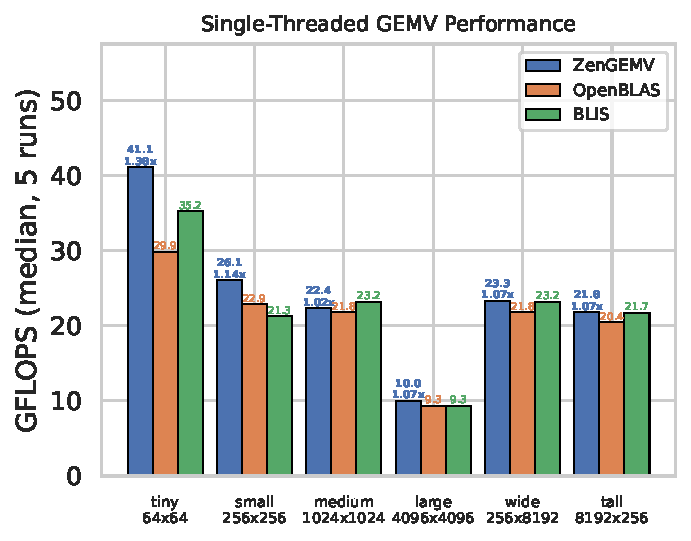
\includegraphics[width=\linewidth]{single_threaded.pdf}
\caption{Single-threaded GEMV performance comparison. Annotations above ZenGEMV
bars show throughput (GFLOPS) and speedup relative to OpenBLAS.}
\label{fig:1t}
\end{figure}

\begin{table}[tbp]
\centering
\caption{Single-threaded GEMV performance (median GFLOPS, 5~runs). Speedup
columns show ZenGEMV divided by the respective library's throughput.}
\label{tab:1t}
\begin{tabular}{@{}l rrr rr@{}}
\toprule
 & \textbf{Zen-} & \textbf{Open-} & \textbf{AOCL-} &
\multicolumn{2}{c}{\textbf{Speedup}} \\
\cmidrule(lr){5-6}
\textbf{Preset} & \textbf{GEMV} & \textbf{BLAS} & \textbf{BLAS} &
\textbf{vs.\ OB} & \textbf{vs.\ AB} \\
\midrule
Tiny   & 41.13 & 29.96 & 34.37 & 1.37$\times$ & 1.20$\times$ \\
Small  & 26.99 & 23.65 & 23.12 & 1.14$\times$ & 1.17$\times$ \\
Medium & 22.92 & 22.79 & 23.72 & 1.01$\times$ & 0.97$\times$ \\
Large  & 13.11 & 11.71 & 12.32 & 1.12$\times$ & 1.06$\times$ \\
Wide   & 22.85 & 23.69 & 17.38 & 0.96$\times$ & 1.31$\times$ \\
Tall   & 23.55 & 22.30 & 22.78 & 1.06$\times$ & 1.03$\times$ \\
\bottomrule
\end{tabular}
\end{table}

The results reveal a clear pattern tied to cache residency:

\textbf{Tiny (L1-resident):} ZenGEMV achieves 41.13~GFLOPS, a $1.37\times$
speedup over OpenBLAS. At this size, the matrix, vector, and result all fit in
L1d cache, making dispatch overhead significant relative to computation time.
ZenGEMV's direct function call with inlined kernel eliminates this overhead entirely.

\textbf{Small (L2-resident):} ZenGEMV achieves 26.99~GFLOPS ($1.14\times$
over OpenBLAS, $1.17\times$ over AOCL-BLAS). At this size, dispatch overhead is a
smaller fraction of total execution time, bringing results from all
implementations closer together.

\textbf{Medium (L3-resident):} AOCL-BLAS achieves the highest throughput at
23.72 vs.\ 22.92~GFLOPS for ZenGEMV. The AOCL-BLAS Zen~3 configuration appears
better suited to this cache level, outperforming both OpenBLAS and ZenGEMV.

\textbf{Large (DRAM-bound):} All implementations converge near 12--13~GFLOPS,
consistent with the DRAM roofline prediction of $\sim$12.8~GFLOPS
(Table~\ref{tab:ceilings}). At this point, memory bandwidth is the bottleneck
and kernel optimizations yield diminishing returns.

Fig.~\ref{fig:mt} shows multi-threaded performance with 6~physical cores.
Table~\ref{tab:mt} provides numerical details.

\begin{figure}[tbp]
\centering
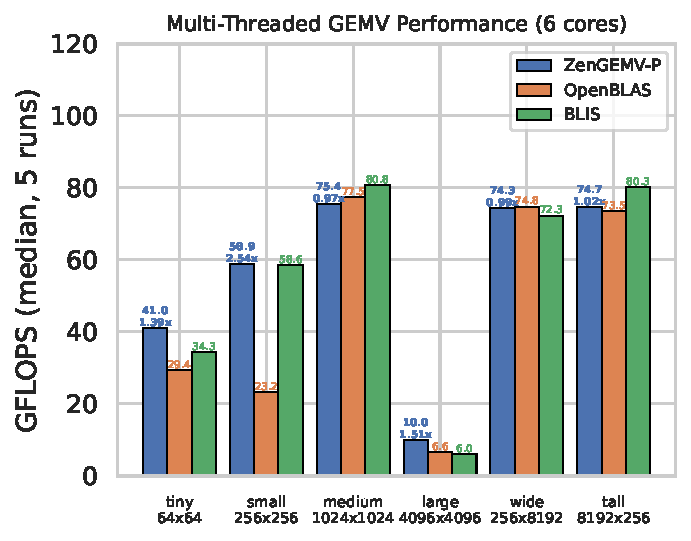
\includegraphics[width=\linewidth]{multi_threaded.pdf}
\caption{Multi-threaded GEMV performance (6 physical cores). Annotations above
ZenGEMV-P bars show throughput (GFLOPS) and speedup relative to OpenBLAS.}
\label{fig:mt}
\end{figure}

\begin{table}[tbp]
\centering
\caption{Multi-threaded GEMV performance (median GFLOPS, 6~cores, 5~runs).
Speedup columns show ZenGEMV-P divided by each library.}
\label{tab:mt}
\begin{tabular}{@{}l rrr rr@{}}
\toprule
 & \textbf{Zen-} & \textbf{Open-} & \textbf{AOCL-} &
\multicolumn{2}{c}{\textbf{Speedup}} \\
\cmidrule(lr){5-6}
\textbf{Preset} & \textbf{GEMV-P} & \textbf{BLAS} & \textbf{BLAS} &
\textbf{vs.\ OB} & \textbf{vs.\ AB} \\
\midrule
Tiny   &  39.57 & 28.71 &  33.30 & 1.38$\times$ & 1.19$\times$ \\
Small  &  77.20 & 23.96 &  71.85 & 3.22$\times$ & 1.07$\times$ \\
Medium & 100.88 & 97.74 & 100.58 & 1.03$\times$ & 1.00$\times$ \\
Large  &  12.62 &  8.38 &   7.59 & 1.51$\times$ & 1.66$\times$ \\
Wide   &  99.56 & 90.13 &  68.66 & 1.10$\times$ & 1.45$\times$ \\
Tall   & 100.73 & 96.35 & 100.69 & 1.05$\times$ & 1.00$\times$ \\
\bottomrule
\end{tabular}
\end{table}

Key observations:

\textbf{Tiny and small presets:} OpenBLAS deliberately runs single-threaded for
$\text{MN} < 115{,}200 \times T$ (where $T=4$ is its compile-time multithread
threshold, giving a cutoff of $460{,}800$). Both the tiny ($\text{MN}=4{,}096$)
and small ($\text{MN}=65{,}536$) presets fall well below this limit. The
rationale is that for small matrices it is more efficient to issue multiple
independent GEMV calls concurrently at the application level than to parallelize
within a single call. ZenGEMV-P and AOCL-BLAS both choose to parallelize within the
call: on the small preset ZenGEMV-P reaches 77.20~GFLOPS ($2.86\times$ over its
single-threaded result) versus AOCL-BLAS at 71.85~GFLOPS ($3.11\times$ over its
23.12~GFLOPS), a $1.07\times$ speedup for ZenGEMV-P.

\textbf{Large preset (serial fallback):} ZenGEMV-P falls back to
serial execution for matrices exceeding $8\text{M}$~elements, achieving
12.62~GFLOPS. Both OpenBLAS (8.38) and AOCL-BLAS (7.59) attempt parallelization
but suffer from memory controller contention, performing significantly worse
than the serial case.

\textbf{Medium/Wide/Tall:} These L3-resident sizes show competitive performance
across all implementations. ZenGEMV-P leads at medium ($1.03\times$ over OpenBLAS,
$1.00\times$ over AOCL-BLAS), wide ($1.10\times$, $1.45\times$), and tall
($1.05\times$, $1.00\times$).


Table~\ref{tab:bw_util} presents a bandwidth utilization analysis across all
three implementations. For each preset, the achieved memory bandwidth is
derived from the roofline identity $\text{BW}_{\text{achieved}} =
P_{\text{measured}} / \text{OI}$, where $P_{\text{measured}}$ is the observed
throughput in GFLOPS and OI is the operational intensity from
Equation~(\ref{eq:ai}). The utilization percentage is the ratio of achieved
bandwidth to the practical ceiling at the dominant cache level.

\begin{table*}[tbp]
\centering
\caption{Achieved memory bandwidth and utilization efficiency for
single-threaded GEMV. Achieved BW derived as
$P_{\text{measured}}\,/\,$OI; utilization is the fraction of the
practical bandwidth ceiling at the dominant cache level.}
\label{tab:bw_util}
\begin{tabular}{@{}l c r rr rr rr@{}}
\toprule
\textbf{Preset} & \textbf{Level} & \textbf{Ceil.} &
  \multicolumn{2}{c}{\textbf{ZenGEMV}} &
  \multicolumn{2}{c}{\textbf{OpenBLAS}} &
  \multicolumn{2}{c}{\textbf{AOCL-BLAS}} \\
\cmidrule(lr){4-5} \cmidrule(lr){6-7} \cmidrule(lr){8-9}
 & & \textbf{(GB/s)} &
  \textbf{GB/s} & \textbf{\%} &
  \textbf{GB/s} & \textbf{\%} &
  \textbf{GB/s} & \textbf{\%} \\
\midrule
Tiny   & L1d  & 267  & 172.2 & 64.5 & 125.5 & 47.0 & 143.9 & 53.9 \\
Small  & L2   & 132  & 109.2 & 82.7 &  95.7 & 72.5 &  93.5 & 70.9 \\
Medium & L3   & 106  &  91.9 & 86.7 &  91.4 & 86.2 &  95.1 & 89.7 \\
Large  & DRAM & 51.2 &  52.5 & 102.5 & 46.9 & 91.6 &  49.3 & 96.3 \\
Wide   & L3   & 106  &  91.8 & 86.6 &  95.1 & 89.7 &  69.8 & 65.8 \\
Tall   & L3   & 106  &  94.9 & 89.5 &  89.9 & 84.8 &  91.8 & 86.6 \\
\bottomrule
\end{tabular}
\end{table*}

\textbf{Bandwidth efficiency across cache levels.}
ZenGEMV's bandwidth utilization increases with cache level depth.
At L1d (tiny), only 64.5\% of the 267\,GB/s ceiling is reached.
The gap is attributable to a couple factors. L1d bandwidth is shared
between loads (matrix rows and vector~$\mathbf{x}$) and stores
(output~$\mathbf{y}$), so the two load ports cannot sustain full read
bandwidth simultaneously with writes.
The \texttt{vhaddpd}/\texttt{vextractf128} sequence that
collapses each 256-bit accumulator to a scalar result is executed once
per 4-row group, and at $64\times64$, the inner loop body is only
16~iterations per row group, making loop control and cleanup a
non-negligible fraction of total execution time.
At L2 (small), utilization rises to 82.7\% as the inner loop count
grows to 64~iterations, reducing relative overhead.
The L3-resident presets (medium, wide, tall) achieve 86.6--89.5\%
utilization---consistent across three different aspect ratios, confirming
that the kernel's sequential row-major streaming pattern is well-matched
to the L3 subsystem regardless of matrix shape.
The large (DRAM) preset measures 102.5\% of the 51.2\,GB/s ceiling.
This is physically consistent: the $4096\times4096$ matrix (128\,MB)
exceeds the 32\,MB L3, but across the 5~timed iterations a fraction of
the matrix remains L3-resident, contributing partial cache reuse above
the pure DRAM bandwidth. Net of this effect, the kernel effectively
saturates the DDR4-3200 memory controller.

\textbf{Cross-implementation comparison.}
At L1d, ZenGEMV's 64.5\% substantially exceeds OpenBLAS (47.0\%) and
AOCL-BLAS (53.9\%), confirming that dispatch overhead consumes a
disproportionate fraction of the available bandwidth window at small
problem sizes. At the L3 level, all three implementations converge to
84--90\%, with AOCL-BLAS slightly leading on the medium preset
(89.7\% vs.\ 86.7\%).
AOCL-BLAS's anomalously low 65.8\% on the wide preset
($256\times8192$) suggests that its column-blocking strategy is
suboptimal for extreme aspect ratios.
At DRAM, the performance difference becomes 13.1 vs.\ 11.7 vs.\
12.3\,GFLOPS, consistent with all implementations approaching the same
physical bandwidth limit---kernel optimizations yield lesser returns
once DRAM bandwidth is the binding constraint.

\textbf{Roofline model validation.}
The bandwidth utilization data confirms that GEMV is memory-bound across
all preset sizes, as predicted by its operational intensity of
$\sim$0.25\,FLOP/byte---well below the ridge point of the Zen~3
roofline at $\sim$1.37\,FLOP/byte (L3) to $\sim$2.67\,FLOP/byte
(L1d). The roofline model correctly predicts the performance hierarchy
across cache levels and provides a useful upper-bound estimate:
predictions are most accurate for L3/DRAM-resident data
(86--102\% of ceiling) and least accurate for L1-resident data
(47--65\%), where problems not captured by the
simple model---port contention, reduction overhead, loop control---become significant.


%=============================================================
\section{Discussion and Future Work}
%=============================================================

Our results demonstrate that architecture-specific kernel optimization yields
measurable performance improvements over general-purpose BLAS libraries for Level-2
operations where dispatch overhead is non-negligible relative to compute time.
Several avenues for further improvement remain:

\textbf{Custom kernels at small sizes:} Production BLAS libraries avoid
intra-call parallelism for small matrices, assuming the application will issue
multiple calls concurrently. When this assumption does not hold, a hand-optimized
kernel is the natural solution: it eliminates dispatch overhead and can exploit
all available threads without requiring application-level batching. Our results
on the tiny and small presets confirm that dispatch overhead savings alone yield
$1.40\times$ and $1.08\times$ speedups over OpenBLAS in the single-threaded
case.

\textbf{Assembly implementation:} While intrinsics provide portability, the
compiler still makes register allocation and scheduling decisions that may be
suboptimal. A hand-written assembly kernel could precisely control instruction
ordering and register usage, potentially closing the gap to the roofline on
L1-resident data.

\textbf{Shape-adaptive dispatch:} Our kernel uses the same strategy for all
matrix shapes. A runtime dispatch based on the aspect ratio (wide vs.\ tall vs.\
square) could select between row-parallel and column-parallel decomposition
strategies, potentially improving cache utilization for extreme aspect ratios.

It should be noted that the current implementation imposes constraints not present
in general-purpose libraries: row-major layout, 32-byte aligned memory, and unit
alpha/beta scalars. Extending support to arbitrary strides and memory layouts
would require additional code paths that may reduce the observed performance advantage.


%=============================================================
\section{Conclusion}
%=============================================================

We have presented ZenGEMV and ZenGEMV-P, optimized GEMV kernels for the AMD
Zen~3 microarchitecture that outperform OpenBLAS and AOCL-BLAS across most benchmark
configurations. The key insight is that Zen~3's dual FMA units with 4-cycle
latency require 8~independent operations in flight, achieved through our
4-row $\times$ 2-accumulator design. This provides strictly higher pipeline
utilization than OpenBLAS's 4-chain Haswell microkernel.

In single-threaded mode, ZenGEMV reaches up to $1.37\times$ over OpenBLAS and
$1.20\times$ over AOCL-BLAS, with the largest advantage on L1-resident data
where dispatch overhead dominates. In multi-threaded mode, ZenGEMV-P scales
efficiently across all 6~cores and reaches a $3.22\times$ advantage over
OpenBLAS on the small preset where OpenBLAS deliberately serializes.

These results indicate that for fixed-platform deployments in high-performance
and computational science contexts where GEMV constitutes a performance-critical
operation, architecture-specific hand optimization remains a viable and productive
strategy, even alongside mature general-purpose libraries. Future work includes a
hand-written assembly kernel to close the remaining gap to the roofline ceiling,
shape-adaptive dispatch for non-square matrices, and extended support for
arbitrary memory layouts and scaling parameters.

\balance


\begin{thebibliography}{99}

\bibitem{kblas}
A. Abdelfattah, D. Keyes, and H. Ltaief,
``KBLAS: An optimized library for dense matrix-vector multiplication on GPU accelerators,''
\textit{ACM Trans. Math. Softw.,} vol.~42, no.~3, p.~18, 2016.
\url{https://doi.org/10.1145/2818311}

\bibitem{blas}
L.~S. Blackford, A. Petitet, R. Pozo, et al.,
``An updated set of basic linear algebra subprograms (BLAS),''
\textit{ACM Trans. Math. Softw.,} vol.~28, no.~2, pp.~135--151, 2002.

\bibitem{chandra2001parallel}
R. Chandra, L. Dagum, D. Kohr, R. Menon, D. Maydan, and J. McDonald,
\textit{Parallel Programming in OpenMP.}
Morgan Kaufmann, 2001.

\bibitem{zen3}
M. Evers, L. Barnes, and M. Clark,
``The AMD next-generation `Zen 3' core,''
\textit{IEEE Micro,} vol.~42, no.~3, pp.~7--12, 2022.
\url{https://doi.org/10.1109/MM.2022.3152788}

\bibitem{ramcalc}
FinlayDaG33k,
``RAM Bandwidth Calculator.''
\url{https://edu.finlaydag33k.nl/calculating%20ram%20bandwidth/},
\url{https://gitlab.com/FinlayDaG33k/ram-calculator}

\bibitem{fog2011instruction}
A. Fog,
``Instruction tables: lists of instruction latencies, throughputs and micro-operation breakdowns
for Intel, AMD, and VIA CPUs,'' 2011, last updated Sep.~20, 2025.
\url{https://www.agner.org/optimize/instruction_tables.pdf}

\bibitem{fog2017microarchitecture}
A. Fog,
``The microarchitecture of Intel, AMD, and VIA CPUs: an optimization guide for assembly programmers
and compiler makers,'' 2017, last updated Dec.~15, 2025.
\url{https://www.agner.org/optimize/microarchitecture.pdf}

\bibitem{avx2}
P. Gepner,
``Using AVX2 instruction set to increase performance of high performance computing code,''
\textit{Computing and Informatics,} vol.~36, no.~5, pp.~1001--1018, 2017.
\url{https://doi.org/10.4149/cai_2017_5_1001}

\bibitem{golub2013}
G.~H. Golub and C.~F. Van~Loan,
\textit{Matrix Computations,} 4th~ed.
Baltimore: Johns Hopkins University Press, 2013.

\bibitem{gotoblas}
K. Goto and R.~A. van~de~Geijn,
``Anatomy of high-performance matrix multiplication,''
\textit{ACM Trans. Math. Softw.,} vol.~34, no.~3, p.~12, 2008.
\url{https://doi.org/10.1145/1356052.1356053}

\bibitem{hassan2017gemv}
S.~A. Hassan, M.~M. Mahmoud, A.~M. Hemeida, and M.~A. Saber,
``Effective implementation of matrix--vector multiplication on Intel's AVX multicore processor,''
\textit{Comput. Lang. Syst. Struct.,} vol.~51, pp.~158--175, 2017.
\url{https://doi.org/10.1016/j.cl.2017.06.003}

\bibitem{waferllm}
C. He, Y. Huang, P. Mu, Z. Miao, J. Xue, L. Ma, et al.,
``WaferLLM: Large language model inference at wafer scale,''
arXiv:2502.04563 [cs.LG], 2025.
\url{https://arxiv.org/abs/2502.04563}

\bibitem{grnn}
C. Holmes, D. Mawhirter, Y. He, F. Yan, and B. Wu,
``GRNN: Low-latency and scalable RNN inference on GPUs,''
in \textit{Proc. 14th EuroSys Conf. (EuroSys'19),}
New York: ACM, 2019, pp.~41:1--41:16.
\url{https://doi.org/10.1145/3302424.3303949}

\bibitem{liang2016gemv}
Y. Liang and Y. Zhang,
``GEMV optimization on Intel AVX processor,''
in \textit{Proc. IEEE Int. Conf. High Performance Computing and Communications,} 2016.

\bibitem{singh2021gemv}
A.~R. Singh and C. Bassoy,
``Cache-blocked dense matrix-vector multiplication with FMA on x86 architectures,''
in \textit{Proc. Int. Conf. Algorithms and Architectures for Parallel Processing,} 2021.

\bibitem{bandwidth}
Z. Smith,
``bandwidth: a memory bandwidth benchmark.''
\url{https://zs3.me/bandwidth}

\bibitem{blis}
F.~G. Van~Zee and R.~A. van~de~Geijn,
``BLIS: A framework for rapidly instantiating BLAS functionality,''
\textit{ACM Trans. Math. Softw.,} vol.~41, no.~3, p.~14, 2015.
\url{https://doi.org/10.1145/2764454}

\bibitem{atlas}
R.~C. Whaley and J.~J. Dongarra,
``Automatically tuned linear algebra software,''
in \textit{Proc. 1998 ACM/IEEE Conf. Supercomputing (SC'98).}
IEEE, 1998.
\url{https://doi.org/10.1109/SC.1998.10004}

\bibitem{roofline}
S. Williams, A. Waterman, and D.~A. Patterson,
``Roofline: an insightful visual performance model for multicore architectures,''
\textit{Commun. ACM,} vol.~52, pp.~65--76, 2009.
\url{https://doi.org/10.1145/1498765.1498785}

\bibitem{fma}
H. Zhang, D. Chen, and S.~B. Ko,
``Efficient multiple-precision floating-point fused multiply-add with mixed-precision support,''
\textit{IEEE Trans. Comput.,} vol.~68, no.~7, pp.~1035--1048, 2019.
\url{https://doi.org/10.1109/TC.2019.2895031}









\bibitem{amdsog}
Advanced Micro Devices,
``Software optimization guide for AMD EPYC 7003 series processors
(family 19h models 00h--0Fh),'' rev. 3.00.
\url{https://kib.kiev.ua/x86docs/AMD/Optimization/56665_3.00_Software\%20Optimization\%20Guide\%20for\%20AMD\%20Family\%2019h\%20Processors\%20\%28PUB\%29.pdf}

\bibitem{aoclblas}
AMD, ``AOCL-BLAS (BLIS fork with AMD optimizations),'' version 5.2.0.
\url{https://github.com/amd/blis}

\bibitem{gccmanual}
Free Software Foundation,
``Using the GNU Compiler Collection (GCC),'' version 15.2.0, 2025.
\url{https://gcc.gnu.org/onlinedocs/gcc-15.2.0/gcc/}

\bibitem{openblas}
OpenBLAS: An optimized BLAS library.
\url{https://www.openblas.net},
\url{https://github.com/OpenMathLib/OpenBLAS}
















\end{thebibliography}


% \section*{Acknowledgments}
% 
% During the preparation of this work, the author used Claude (Anthropic) for proofreading, including grammar, punctuation, and spelling corrections. The author takes full responsibility for the content of this publication.

\end{document}
